\documentclass[11pt,a4paper,oldfontcommands,openany]{memoir}
\usepackage{graphicx}
\usepackage[]{color}
\usepackage{courier}
\usepackage[usenames,dvipsnames]{xcolor}
\usepackage[breakable, theorems, skins]{tcolorbox}
\usepackage[]{media9}
\usepackage{lipsum}

\usepackage{lineno} %% LINE COUNTS
\linenumbers %% LINE COUNTS

\tcbset{enhanced}
%% maxwidth is the original width if it is less than linewidth
%% otherwise use linewidth (to make sure the graphics do not exceed the margin)
\makeatletter
\def\maxwidth{ %
  \ifdim\Gin@nat@width>\linewidth
    \linewidth
  \else
    \Gin@nat@width
  \fi
}
\makeatother

\DeclareRobustCommand{\mybox}[2][gray!15]{%
\begin{tcolorbox}[   %% Adjust the following parameters at will.
        breakable,
        left=0pt,
        right=0pt,
        top=0pt,
        bottom=0pt,
        colback=#1,
        colframe=#1,
        width=\dimexpr\textwidth\relax, 
        enlarge left by=0mm,
        boxsep=5pt,
        arc=0pt,outer arc=0pt,
        ]
        #2
\end{tcolorbox}
}


\definecolor{fgcolor}{rgb}{0.345, 0.345, 0.345}
\newcommand{\hlnum}[1]{\textcolor[rgb]{0.686,0.059,0.569}{#1}}%
\newcommand{\hlstr}[1]{\textcolor[rgb]{0.192,0.494,0.8}{#1}}%
\newcommand{\hlcom}[1]{\textcolor[rgb]{0.678,0.584,0.686}{\textit{#1}}}%
\newcommand{\hlopt}[1]{\textcolor[rgb]{0,0,0}{#1}}%
\newcommand{\hlstd}[1]{\textcolor[rgb]{0.345,0.345,0.345}{#1}}%
\newcommand{\hlkwa}[1]{\textcolor[rgb]{0.161,0.373,0.58}{\textbf{#1}}}%
\newcommand{\hlkwb}[1]{\textcolor[rgb]{0.69,0.353,0.396}{#1}}%
\newcommand{\hlkwc}[1]{\textcolor[rgb]{0.333,0.667,0.333}{#1}}%
\newcommand{\hlkwd}[1]{\textcolor[rgb]{0.737,0.353,0.396}{\textbf{#1}}}%

\usepackage{framed}
\makeatletter
\newenvironment{kframe}{%
 \def\at@end@of@kframe{}%
 \ifinner\ifhmode%
  \def\at@end@of@kframe{\end{minipage}}%
  \begin{minipage}{\columnwidth}%
 \fi\fi%
 \def\FrameCommand##1{\hskip\@totalleftmargin \hskip-\fboxsep
 \colorbox{shadecolor}{##1}\hskip-\fboxsep
     % There is no \\@totalrightmargin, so:
     \hskip-\linewidth \hskip-\@totalleftmargin \hskip\columnwidth}%
 \MakeFramed {\advance\hsize-\width
   \@totalleftmargin\z@ \linewidth\hsize
   \@setminipage}}%
 {\par\unskip\endMakeFramed%
 \at@end@of@kframe}
\makeatother

\definecolor{shadecolor}{rgb}{.97, .97, .97}
\definecolor{messagecolor}{rgb}{0, 0, 0}
\definecolor{warningcolor}{rgb}{1, 0, 1}
\definecolor{errorcolor}{rgb}{1, 0, 0}
\newenvironment{knitrout}{}{} % an empty environment to be redefined in TeX

\usepackage{alltt}
\setlength{\parindent}{0pt} % Remove indent at new paragraphs
\setcounter{secnumdepth}{4}  % Remove section numbering at certain depth # If zero, then no numbering of sections
\setcounter{tocdepth}{4} % Determines number of subsections that will have tabs
\usepackage{tabu}
\usepackage{url}

\usepackage[round]{natbib}   % omit 'round' option if you prefer square brackets
\bibliographystyle{plainnat}

\usepackage{fixltx2e}
%\usepackage{graphicx}	% For external pictures
\usepackage{float}
\usepackage{subfig}	% Add subfigures within figures
\usepackage{verbatim}
\usepackage[colorlinks=true,linkcolor=blue,citecolor=blue,urlcolor=blue]{hyperref}
\usepackage{amssymb,amsbsy,amsmath}
\usepackage{epsfig}
\usepackage[left=3cm,top=3cm,bottom=3.5cm,right=3cm]{geometry} % For easy document margins
%\usepackage{fancyhdr} % For customization of header/footer
\usepackage{adjustbox}
\usepackage{framed}
\usepackage{enumitem}
\usepackage{caption}
\numberwithin{equation}{section} % Equation numbers relative to sections

%%%%% NEW ADDED FROM THESIS.TEX %%%%% 
\usepackage[utf8]{inputenc}
\usepackage[T1]{fontenc}
\usepackage{microtype}
%\usepackage[dvips]{graphicx}
%\usepackage{times} %clash
%%%%%%%%%%%%%%%%%%%%%%%%%%%%%%%%%%%%%%%% 
\newcommand{\code}[1]{{\texttt{#1}}}
\newcommand{\pkg}[1]{{\texttt{#1}}}
\newcommand{\class}[1]{{\textit{#1}}}
\newcommand{\R}{{\normalfont\textsf{R }}{}}
\IfFileExists{upquote.sty}{\usepackage{upquote}}{}


\begin{document}

\sloppy

%%%%%%%%%%%%%%%%%%%%% TITLE PAGE %%%%%%%%%%%%%%%%%%%%%

% {
% \centering
% ~\vspace{\fill}
% 
% \vspace{2.5cm}
% 
% {\LARGE Thesis Proposal}
% 
% \vspace{1cm}
% 
% {\LARGE\textbf{Visualization methods for genealogical and RNA-sequencing datasets}}
% 
% \vspace{1cm}
% 
% {\LARGE Lindsay Rutter}
% 
% \vspace{4cm}
% 
% {\LARGE Program of Study Committee:}
% 
% \vspace{1cm}
% 
% {\LARGE Dianne Cook (Major Professor)}
% 
% \vspace{.25cm}
% 
% {\LARGE Amy Toth (Major Professor)}
% 
% \vspace{.25cm}
% 
% {\LARGE Heike Hofmann}
% 
% \vspace{.25cm}
% 
% {\LARGE Daniel Nettleton}
% 
% \vspace{.25cm}
% 
% {\LARGE James Reecy}
% 
% \vspace{2.5cm}
% 
% {\centerline{\large May 16, 2016}}
% }
% 
% \clearpage
%\cleardoublepage

%%% CHAPTER'S STYLE
\chapterstyle{bianchi}
\setsecheadstyle{\Large\bfseries\sffamily\raggedright}
\setsubsecheadstyle{\large\bfseries\sffamily\raggedright}
\setsubsubsecheadstyle{\bfseries\sffamily\raggedright}
%%%%%%%%%%%%%%%%%%%%%%%%%%%%%%%%%%%%

%\tableofcontents

\setlength{\parskip}{10pt} % Inter-paragraph spacing

%%% ADDED FROM THESIS.TEX %%%%%%%%%
\OnehalfSpacing

\chapter{Gene expression responses to diet quality and viral infection in \textit{Apis mellifera}}

\section{Introduction}

Commerically managed honeybees have undergone unusually large declines in the United States and parts of Europe over the past decade (\citealt{ccd1}, \citealt{ccd2}, \citealt{ccd3}), with annual mortality rates exceeding what beekeepers consider sustainable (\citealt{ccd5}, \citealt{ccd6}). More than 70 percent of major global food crops (including fruits, vegatables, and nuts) at least benefit from pollination, and yearly insect pollination services are valued wordwide at \$175 billion (\citealt{ccd7}). As honeybees are largely considered to be the leading pollinator of numerous crops, their marked loss has considerable implications regarding agricultural sustainability (\citealt{ccd4}).

Honeybee declines have been associated with several factors, including pesticide use, parasites, pathogens, habitat loss, and poor nutrition (\citealt{factors}, \citealt{factors2}). Researchers generally agree that these stressors do not act in isolation; instead, they appear to influence the large-scale loss of honeybees in interactive fashions as the environment changes (\citealt{interacting}). Nutrition and viral infection are two broad factors that pose heightened dangers to honeybee health in response to recent environmental changes.

Pollen is the main source of nutrition (including proteins, amino acids, lipids, sterols, starch, vitamins, and minerals) in honeybees (\citealt{source}, \citealt{source2}). At the individual level, pollen supplies most of the nutrients necessary for physiological development (\citealt{brodschneider}) and is believed to have considerable impact on longevity (\citealt{longevity}). At the colony level, pollen enables young workers to produce jelly, which then nourishes larvae, drones, older workers, and the queen (\citealt{jelly}, \citealt{jelly2}). Various environmental changes (including urbanization and monoculture crop production) have significantly altered the nutritional profile available to honeybees. In particular, honeybees are confronted with less diverse selections of pollen, which is of concern because mixed-pollen (polyfloral) diets are generally considered healthier than single-pollen (monofloral) diets (\citealt{diverse}, \citealt{diverse2}, \citealt{alaux}). Indeed, reported colony mortality rates are higher in developed land areas compared to undeveloped land areas (\citealt{undeveloped}), and beekeepers rank poor nutrition as one of the main reasons for colony losses (\citealt{bkLoss}). Understanding how undiversified diets affect honeybee health will be crucial to resolve problems that may arise as agriculture continues to intensify throughout the world (\citealt{ag}, \citealt{ag2}).

Viral infection was a comparatively minor problem in honeybees until the last century when Varroa destructor (an ectoparasitic mite) spread worldwide (\citealt{miteSpread}). This mite feeds on honeybee hemolymph (\citealt{hemolymph}), transmits cocktails of viruses, and supports replication of certain viruses (\citealt{miteVirus}, \citealt{miteVirus2}, \citealt{miteVirus3}). More than 20 honeybee viruses have been identified (\citealt{numVirus}). One of these viruses that has been linked to honeybee decline is Israeli Acute Paralysis Virus (IAPV). A positive-sense RNA virus of the Dicistroviridae family (\citealt{fam}), IAPV causes infected honeybees to display shivering wings, decreased locomotion, muscle spams, and paralysis, and 80\% of caged infected adult honeybees die prematurely (\citealt{symptoms}). IAPV has demonstrated higher infectious capacities than other honeybee viruses in certain conditions (\citealt{carrillo}) and is more prevalent in colonies that do not survive the winter (\citealt{winter}). Its role in the rising phenomenon of ``Colony Collapse Disorder'' (in which the majority of worker bees disappear from a hive) remains unclear: It has been implicated in some studies (\citealt{iapvCCD}, \citealt{iapvCCD2}) but not in other studies (\citealt{ccd1}, \citealt{iapvCCD3}, \citealt{fam}). Nonetheless, it seems likely that IAPV reduces colony strength and survival.

Although there is growing interest in how viruses and diet quality affect the health and sustainability of honeybees, as well as a recognition that such factors might operate interactively, there are only a small number of experimental studies thus far directed toward elucidating the interactive effects of these two factors in honeybees (\citealt{intNV}, \citealt{intNV2}, \citealt{intNV3}). We recently used laboratory cages and nucleus hive experiments to investigate the health effects of these two factors, and our results show a significant interaction between diet quality and virus infection. Specifically, high quality pollen is able to mitigate virus-induced mortality to the level of diverse, polyfloral pollen (\citealt{adamInt}). 

Following up on these phenotypic findings from our previous study, we now aim to understand the corresponding underlying mechanisms by which high quality diets protect bees from virus-induced mortality. For example, it is not known whether the protective effect of good diet is due to direct, specific effects on immune function (resistance), or if it is due to indirect effects of good nutrition on energy availability/vigor (resilience). Transcriptomics is one means to achieve this goal. Transcriptomic analysis can help to identify 1) the genomic scale of transcriptomic response to diet and virus infection, 2) whether these factors interact in an additive or synergistic way on transcriptome function, and 3) the types of pathways affected by diet quality and viral infection. This information, heretofore lacking in the literature, can help us to better understand how good nutrition may be able to serve as a "buffer" against other stressors (\citealt{AdamTothReview}). As it stands, there are only a small number of published experiments examining gene expression patterns related to diet effects (\citealt{alaux2}) and IAPV infection effects (\citealt{galbraith}) in honeybees. As far as we know, there are few to no studies investigating honeybee gene expression patterns specifically related to monofloral diets, and few to no studies investigating gene expression patterns related to the interaction effects of diet in any broad sense and viral innoculation in any broad sense in honeybees. 

In this study, we examine how monofloral diets and viral innoculation influence gene expression patterns in honeybees by focusing on four treatment groups (low quality diet without IAPV exposure, high quality diet without IAPV exposure, low quality diet with IAPV exposure, and high quality diet with IAPV exposure). We conduct RNA-sequencing analysis on a randomly selected subset of the honeybees we used in our previous study (as is further described in our methods section). We then examine pairwise combinations of treatment groups, the main effect of monofloral diet, the main effect of IAPV exposure, and the interactive effect of the two factors on gene expression patterns.

We also compare the main effect of IAPV exposure in our dataset to that obtained in a previous study conducted by Galbraith and colleagues (\citealt{galbraith}). As RNA-sequencing data can be highly noisy, this comparison allowed us to characterize how repeatable and robust our RNA-seq results were in comparison to previous studies. Importantly, we use an in-depth data visualization approach to explore and validate our data, and suggest such an approach can be useful for cross-study comparisons of RNA-sequencing data in the future.

\section{Methods}

Details of the procedures we used to prepare virus inoculum, infect and feed caged honeybees, and quantify IAPV can be reviewed in our previous work (\citealt{adamInt}). The statistical analysis we used to study the main and interaction effects of the two factors on mortality and IAPV titers is also described in our earlier report (\citealt{adamInt}).

\subsection{Design of diet experiment}

There are several reasons why, in this part of our previous study, we focused only on diet quality (monofloral diets) as opposed to diet diversity (monofloral diets versus polyfloral diets). First, when assessing diet diversity, a sugar diet is often used as a control. However, such an experimental design does not reflect real-world conditions for honeybees as they rarely face a total lack of pollen (\citealt{DiPasquale}). Second, in studies that compared honeybee health using monofloral and polyfloral diets at the same time, if the polyfloral diet and one of the high-quality monofloral diets both exhibited similarly beneficial effects, then it was difficult for the authors to assess if the polyfloral diet was better than most of the monofloral diets because of its diversity or because it contained as a subset the high-quality monofloral diet (\citealt{DiPasquale}). Third, colonies used for pollination in agricultural areas (monoculture) face less diversified pollens (according to Brodschneider, 2010). Pollinating areas are currently undergoing landscape alteration and agriculture intensification, and bees are increasingly faced wtih less diversified diets (monoculture) (\citealt{landscape1}, \citealt{brodschneider}). As a result, there is a need to better understand how monofloral diets affect honeybee health as a step toward mitigating the negative impact of human activity on the honeybee population.

Consequently, in our prior study, for our nutrition factor, we examined two monofloral pollen diets, Cistus (Rockrose) and Castanea (Chestnut). Cistus pollen is generally considered less nutritious than Castanea pollen due to its lower levels of protein, amino acids, antioxidants, calcium, and iron (\citealt{DiPasquale}, \citealt{adamInt}). For our virus factor, one level contained bees that were infected with IAPV and another level contained bees that were not infected with IAPV. This experimental design resulted in four treatment groups (Cistus pollen without IAPV exposure, Castanea pollen without IAPV exposure, Cistus pollen with IAPV exposure, and Castanea pollen with IAPV exposure) that allowed us to assess main effects and interactive effects between diet quality and IAPV infection in honeybees.

\subsection{RNA extraction}

Fifteen cages per treatment were originally sampled. Six live honeybees from each cage were randomly selected 36 hours post inoculation and placed into tubes. Tubes were kept on dry ice and then transferred into a -80C freezer until processing. Eight cages were randomly selected from the original 15 cages, and 2 honeybees per cage were randomly selected from the original six live honeybees per cage. Whole body RNA from each pool of two honeybees were extracted using Qiagen RNeasy MiniKit followed by Qiagen DNase treatment. Samples were suspended in water to 200-400 ng/$\mu$l. All samples were then tested on a Bioanalyzer at the DNA core facility to ensure quality (RIN>8).

\subsection{Gene expression}

Samples were sequenced starting on January 14, 2016 at the Iowa State University DNA Facility (Platform: Illumina HiSeq Sequencing; Category: Single End 100 cycle sequencing). A standard Illumina mRNA library was prepared by the DNA facility. Reads were aligned to the BeeBase Version 3.2 genome (\citealt{hbGenome}) from the Hymenoptera Genome Database (\citealt{hymenopteraDB}) using the programs GMAP and GSNAP (\citealt{gsnap}). We tested all six pairwise combinations of treatments for DEGs (pairwise DEGs). We also tested the diet main effect (diet DEGs), virus main effect (virus DEGs), and interaction term for DEGs (interaction DEGs). We then also tested for virus main effect DEGs (virus DEGs) in public data derived from a previous study exploring the gene expression of IAPV virus infection in honeybees (\citealt{galbraith}). We tested each DEG analysis using recommended parameters with DESeq2 (\citealt{deseq2}), edgeR (\citealt{edger}), and LimmaVoom (\citealt{limma}). In all cases, we used a false discovery rate (FDR) threshold of 0.05 (\citealt{benjamini}). Fisher's exact test was used to determine significant overlaps between DEG sets (whether from the same dataset but across different analysis pipelines or from different datasets across the same analysis pipelines). 

@@@ What percent of reads mapped?
@@@ Total number of raw reads
@@@ How many lanes
@@@ How many samples per lane

\subsection{Comparison to previous studies on transcriptomic response to viral infection}

We also compare the main effect of IAPV exposure in our dataset to that obtained in a previous study conducted by Galbraith and colleagues (\citealt{galbraith}). While our study examines honeybees from polyandrous colonies, the Galbraith study examined honeybees from single-drone colonies. As a consequence, our honeybees will have an average of about 75\% genetic variance, and the honeybees from the Galbraith study will have an average of about 25\% genetic variance (\citealt{sisters}). We should therefore expect that the Galbraith study may generate data with lower signal:to:noise ratios than our data due to the lower genetic variation between its replicates. At the same time, our honeybees will be more likely to display the health benefits gained from increased genotypic variance within colonies, including decreased parasitic load (\citealt{multParasite}), increased tolerance to environmental changes (\citealt{divHyp2}), and increasead colony performance (\citealt{geneticDiverse}, \citealt{geneticDiverse2}). Given that honeybees are naturally very polyandrous (\citealt{patriline}), our honeybees may also reflect more realistic environmental and genetic simulations. Taken together, each study provides a different point of value: Our study likely presents less artificial data while the Galbraith data likely presents less messy data. We wish to explore how the gene expression effects of IAPV innoculation compare between these two studies that used such different experimental designs. To achieve this objective, we use visualization techniques to assess the signal:to:noise ratio between these two datasets, and differential gene expression (DEG) analyses to determine any significantly overlapping genes of interest between these two datasets. It is our hope that this aspect of our study may shine light on how experimental designs that control genetic variability to different extents might affect the resulting gene expression data in honeybees.

\subsection{Visualization}

We used @@@ visualization tools from @@@ and visual inference techniques to assess the signal:to:noise ratio in the datasets and to assess the suitability of the DEG calls. 

\subsection{Gene Ontology}

DEGs were uploaded as a background list to DAVID Bioinformatics Resources 6.7 (\citealt{davidBio}, \citealt{davidBio2}). The overrepresented gene ontology (GO) terms of DEGs were identified using the BEEBASE\_ID identifier. To fine-tune the GO term list, only significant terms (FDR < 0.05) and those correlating to Biological Processes were considered. The refined GO term list was then imported into REVIGO (\citealt{revigo}), which uses semantic similarity measures to cluster long lists of GO terms.

\section{Results}

\subsection{Phenotypic results}

We reanalyzed our previously published dataset with a subset more relevant to our RNA-sequencing approaches in the current study that have a more focused question regarding diet quality. We briefly show it again here to inform the RNA-seq comparison because we reduced the number of treatments (from eight to four) from the original published data (\citealt{adamInt}). When statistically analyzing the subset of this data that was used for RNA-sequencing analysis, we found that the mortality rates across diet quality and virus exposure at least numerically retained the same trends (Figure \ref{fig:4panels}).

Mortality rates of honeybees 72 hour post-inoculation differed (or did not?) among the treatment groups (mixed model ANOVA across all treatment groups, df=@@@, @@@; F=@@@; p<@@@). The effect of virus treatment (mixed model ANOVA, df=@@@, @@@; F=@@@; p<@@@), diet treatment (mixed model ANOVA, df=@@@,@@@; F=@@@; p<@@@), and interaction between the two factors (mixed model ANOVA, df=@@@, @@@; F=@@@, p=@@@) did (or did not?) differ. The virus treatment was significant: For a given diet, honeybees exposed to the virus showed significantly higher mortality rate than honeybees not exposed to the virus (Tukey HSD, p<0.05). Without virus exposure, there was only an intermediate reduction in mortality rate for bees fed Castanea pollen? (Tukey HSD, p>0.05). However, with virus exposure, there was a significant reduction in mortality rate for beeds fed Castanea pollen (Tukey HSD, p<0.05). Overall, we discovered that the higher-quality Castanea diet had the ability to significantly reduce mortality in the presence of IAPV infection compared to the lower-quality Cistus diet (Figure \ref{fig:4panels}).

Comment on (Figure \ref{fig:4panels}) @@@

\begin{figure}[H]
\centering
  \begin{framed}
  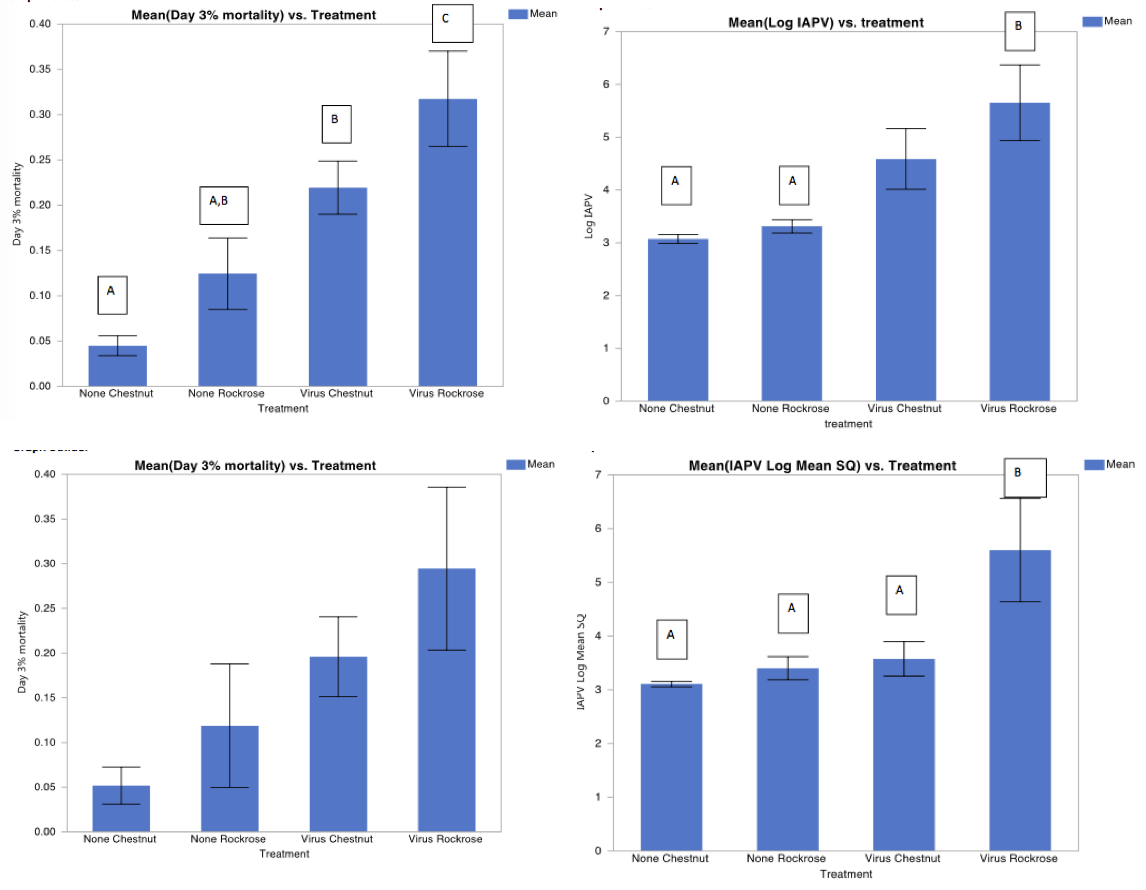
\includegraphics[width=0.8\textwidth]{Images/4panels}
  \end{framed}
  \caption{Mortality rates for all cages, mortality rates for subset of honeybees used for RNA-seq, IAPV titers for all cages, IAPV titers for subset of honeybees used for RNA-seq subset.}
  \label{fig:4panels}
\end{figure}


\section{Discussion}




% SYNTAX
%%%%%%%%%%%%%%%%%%%%%%%%%%%%%%%%%%%%%%%%%%%%%%%%%%%%%%%%%
%%%%%%%%%%%%%%%%%%%%%%%%%%%%%%%%%%%%%%%%%%%%%%%%%%%%%%%%%

%\ref{sec:ggenealogy}
% \code{ggparcoord}
% \Figure \ref{fig:porcupine}

% \begin{figure}[H]
% \centering
%     \begin{framed}
%     \includegraphics[width=0.8\textwidth]{porcupine}
%     \end{framed}
%     \caption{Three}
%     \label{fig:porcupine}
% \end{figure}

% \section{Literature review}
% \label{sec:litReview}

% \pkg{R} statistical programming language allows for tools to be distributed and modified at ease, encourages cross-platform collaboration, and provides a foundation for effective and aesthetic data visualization from the grammar of graphics. There are several useful \pkg{R} packages that offer tools for analyzing and visualizing genealogical datasets. Here, we introduce these packages, and emphasize the shortcomings for which our package \pkg{ggenealogy} brings to this collection of work.

%\clearpage

%\begin{enumerate}
%\item The data can be viewed at \url{http://shiny.soybase.org/CNV/}.
%\end{enumerate}

% \begin{tabular}{|p{2.6cm}|p{5.65cm}|p{5.65cm}|}
%  \hline
%  & \textbf{Drumming Treatment (D)} & \textbf{No Drumming Treatment (N)} \\ 
%  \hline
%  \textbf{Restricted} & \textbf{DR} & \textbf{NR} \\ 
%  \textbf{Nutrition (R)}& Predict most worker-like & Predict some worker-like \\
%  & gene expression & gene expression \\
%  \hline
%  \textbf{Unrestricted} & \textbf{DU} & \textbf{NU} \\ 
%  \textbf{Nutrition (U)} & Predict some worker-like & Predict least worker-like \\
%  & gene expression & gene expression \\
%  \hline
% \end{tabular}

\bibliography{chapter4}

\end{document}
